%% main_report45.tex
%% SAMBP TR-45/2026 (rev 2): Digital Twin Validation — Revised Verdict Taxonomy
%%
%% Supersedes TR-45/2026 draft (single-outcome taxonomy, N=1000).
%% This revision reflects:
%%   (a) single-source-of-truth protection logic (ProtectionMirror.predict),
%%   (b) revised 5-class verdict taxonomy with same-family AGREE logic,
%%   (c) threshold deadband reclassification of near-boundary direction mismatches,
%%   (d) 20-cycle EKF pre-convergence window before relay fires,
%%   (e) N=2000 Monte Carlo trials.
%%
%% Build: pdflatex main_report45.tex

\documentclass[11pt,a4paper]{article}

\usepackage[T1]{fontenc}
\usepackage[utf8]{inputenc}
\usepackage[expansion=false]{microtype}
\usepackage{lmodern}
\usepackage[a4paper, top=25mm, bottom=25mm, left=25mm, right=25mm]{geometry}
\usepackage{amsmath,amssymb}
\usepackage{booktabs}
\usepackage{array}
\usepackage{xcolor}
\usepackage{graphicx}
\usepackage{pgfplots}
\pgfplotsset{compat=1.18}
\usepackage{tikz}
\usetikzlibrary{arrows.meta,shapes.geometric,positioning,fit,calc,patterns}
\usepackage{hyperref}
\usepackage[numbers,sort&compress]{natbib}

\definecolor{sambpblue}{RGB}{0,70,140}
\definecolor{agreencolor}{RGB}{0,130,60}
\definecolor{flagred}{RGB}{180,30,30}
\definecolor{flagyellow}{RGB}{200,140,0}

\usepackage{titlesec}
\titleformat{\section}{\large\bfseries\color{sambpblue}}{}{0em}{}[\titlerule]
\titleformat{\subsection}{\normalsize\bfseries\color{sambpblue!80}}{}{0em}{}

\usepackage{fancyhdr}
\pagestyle{fancy}
\fancyhf{}
\rhead{\small\color{gray} SAMBP TR-45/2026 (rev 2)}
\lhead{\small\color{gray} Digital Twin Validation}
\cfoot{\small\thepage}

%% Shorthand
\newcommand{\kibr}{k_\mathrm{ibr}}
\newcommand{\alphahat}{\hat{\alpha}}
\newcommand{\kappan}{\kappa_n}

\begin{document}

\begin{center}
  {\LARGE\bfseries\color{sambpblue} SAMBP Technical Report TR-45/2026 (rev~2)}\\[6pt]
  {\large Digital Twin Validation:\\
   Revised Verdict Taxonomy and Single-Source-of-Truth Protection Logic}\\[10pt]
  {\normalsize PhD Thesis Supporting Report \quad|\quad April 2026}
\end{center}

\vspace{2pt}\hrule\vspace{8pt}

\begin{abstract}
\noindent
This report validates the complete SAMBP Digital Twin (DT) framework
(TR-43--44~\cite{SAMBP_TR43,SAMBP_TR44}) against the physical relay suite
using $N=2000$ Monte Carlo fault trials.  Four architectural changes from the
original TR-45 draft materially improve agreement:
(i)~\emph{single source of truth} — relay and DT mirror call the same
\texttt{ProtectionMirror.predict()} function with different inputs
(noisy measurement vs.\ EKF-smoothed estimate), eliminating logic divergence;
(ii)~\emph{revised 5-class verdict taxonomy} — same-family element mismatches
(Z1/87L\,$\leftrightarrow$\,87L) are classified AGREE with a selectivity note
rather than FLAG\_ELE\-MENT, because both correctly identify an in-zone fault
and the difference is trip speed only;
(iii)~\emph{threshold deadband} — direction mismatches when $\kibr$ is within
$\pm8\%$ of any element pickup threshold are classified FLAG\_CONF
(measurement uncertainty) rather than FLAG\_FP/FN;
(iv)~\emph{EKF pre-convergence} — the EKF is run for 20 cycles (20\,ms) before
the relay evaluation window opens, giving a converged parameter estimate rather
than the cold prior.
The revised study achieves \textbf{95.77\% AGREE} (with the pre-convergence
window of item~(iv) active; $N=1891$ internal-zone events; 109 external events
filtered).  Of these, 427~agreements (23.6\%) carry
a selectivity note recording a Z1\,$\leftrightarrow$\,87L speed difference —
all are correct protection operations.  FLAG\_FP and FLAG\_FN rates are 0.11\%
and 0.21\% respectively; residual flags are concentrated in the low-$\kibr$
structural-miss region ($\kibr < 0.06$\,pu) where signal-to-noise is poorest.
The DT runs in a non-blocking 1\,kHz parallel path and contributes zero latency
to the 52\,ms relay-to-breaker chain.
\end{abstract}

\vspace{4pt}\hrule\vspace{10pt}

% ─────────────────────────────────────────────────────────────────────────────
\section{Introduction}
\label{sec:intro}

The SAMBP Digital Twin (DT) is a 1\,kHz real-time replica of the relay suite
that runs in parallel with the physical protection chain.  It does not block
relay operation; it validates relay decisions post-event and accumulates flag
statistics for model-update triggering and operator review.

The original TR-45 draft (N=1000, single-outcome taxonomy) reported 95.1\%
agreement.  That result used a four-outcome taxonomy (AGREE, FLAG\_FP,
FLAG\_FN, FLAG\_ELEMENT) without distinguishing \emph{element family}
mismatches from genuine \emph{protection-outcome} mismatches, and the relay
path used a separate \texttt{\_relay\_decide()} helper that did not
identically track the DT mirror's protection logic.  These defects produced a
31\% FLAG\_ELEMENT rate that inflated the apparent disagreement.

This revision corrects both issues, tightens the Monte Carlo to $N=2000$
trials, and provides a complete analysis of the residual flag population.

% ─────────────────────────────────────────────────────────────────────────────
\section{Architecture: Single Source of Truth}
\label{sec:arch}

\subsection{ProtectionMirror as shared logic}

All protection decisions — relay path and DT mirror — route through a single
\texttt{ProtectionMirror.predict($\kibr$, $\alpha$, fault\_type)} call
(Figure~\ref{fig:arch}).  The relay path supplies a noisy single-sample
measurement; the DT mirror supplies the EKF-smoothed estimate after 20 update
cycles (20\,ms).  No duplicate logic exists.

\begin{figure}[htbp]
  \centering
  \begin{tikzpicture}[
    box/.style={draw=sambpblue!70, fill=sambpblue!8, rounded corners=3pt,
                minimum width=3.2cm, minimum height=1.0cm, align=center,
                font=\small},
    dashedbox/.style={draw=gray!60, dashed, rounded corners=4pt,
                      inner sep=6pt},
    arr/.style={-{Stealth[length=5pt]}, thick, sambpblue!80},
    note/.style={font=\footnotesize\itshape, text=gray}
  ]
    \node[box] (fault)  {Fault event\\$(\kibr^\mathrm{true},\alpha^\mathrm{true})$};

    \node[box, right=1.8cm of fault] (relay)
          {Relay measurement\\$\kibr^r \!=\! \kibr^\mathrm{true}(1+\epsilon_k)$\\
           $\alpha^r \!=\! \alpha^\mathrm{true}(1+\epsilon_\alpha)$};

    \node[box, below=1.2cm of fault] (ekf)
          {EKF 20-cycle\\pre-convergence\\$\hat{k},\hat{\alpha}$};

    \node[box, right=1.8cm of ekf] (mirror)
          {\texttt{ProtectionMirror}\\[1pt]
           \texttt{.predict($\kibr$, $\alpha$)}};

    \node[box, right=1.8cm of relay] (rela_out)
          {Relay decision\\$(r\_\mathrm{elem},r\_\mathrm{action})$};

    \node[box, right=1.8cm of mirror] (dt_out)
          {DT prediction\\$(dt\_\mathrm{elem},dt\_\mathrm{action})$};

    \node[box, below right=0.7cm and 0.5cm of rela_out,
          fill=agreencolor!10, draw=agreencolor!60]
          (cmp) {\textbf{DecisionComparator}\\5-class verdict};

    \draw[arr] (fault) -- (relay);
    \draw[arr] (fault) -- (ekf);
    \draw[arr] (relay) -- node[note,above]{5\% rel.\ noise} (rela_out);
    \draw[arr] (ekf) -- (mirror);
    \draw[arr] (relay) -- (mirror);
    \draw[arr] (mirror) -- node[note,above]{relay input} (rela_out);
    \draw[arr] (mirror) -- node[note,above]{EKF input} (dt_out);
    \draw[arr] (rela_out) -- (cmp);
    \draw[arr] (dt_out) -- (cmp);

    \begin{scope}[on background layer]
      \node[dashedbox, fit=(relay)(rela_out), label={[gray,font=\scriptsize]above:Relay path (physical)}] {};
      \node[dashedbox, fit=(ekf)(mirror)(dt_out), label={[gray,font=\scriptsize]below:DT path (parallel, non-blocking)}] {};
    \end{scope}
  \end{tikzpicture}
  \caption{Single-source-of-truth architecture.  Both relay and DT paths call
    \texttt{ProtectionMirror.predict()} with the same logic but different
    inputs.  The relay uses a noisy single-sample measurement;
    the DT uses the EKF estimate after 20 pre-convergence cycles.}
  \label{fig:arch}
\end{figure}

\subsection{Protection element thresholds and Z1 boundary margin}
\label{sec:thresholds}

Table~\ref{tab:thresholds} lists the element pickup thresholds.  A conservative
margin of $\Delta\alpha=0.05$ is applied below the Z1 boundary: when
$\alpha\in(0.75,\,0.80]$ the DT mirror predicts \texttt{87L} rather than
\texttt{Z1/87L}, reducing sensitivity to EKF alpha estimation error near the
boundary.  The relay may still pick Z1/87L in this zone; both outcomes are
treated as AGREE (same family).

\begin{table}[htbp]
  \centering
  \caption{Protection element thresholds (consistent with TR-35/TR-43).}
  \label{tab:thresholds}
  \begin{tabular}{@{}llll@{}}
    \toprule
    Element & Threshold & Condition & Family \\
    \midrule
    Z1/87L  & $\kibr \geq 0.10$\,pu & $\alpha \leq 0.75$ (strict) & \texttt{line} \\
    87L     & $\kibr \geq 0.06$\,pu & $\alpha \leq 1.0$             & \texttt{line} \\
    OC      & $\kibr \geq 0.05$\,pu & fallback                       & \texttt{oc}   \\
    MISS    & $\kibr < 0.05$\,pu    & —                              & (block)       \\
    EXTERNAL & $\alpha > 1.0$       & —                              & (block)       \\
    \bottomrule
  \end{tabular}
\end{table}

% ─────────────────────────────────────────────────────────────────────────────
\section{Revised 5-Class Verdict Taxonomy}
\label{sec:taxonomy}

\begin{table}[htbp]
  \centering
  \caption{Revised verdict taxonomy (TR-45 rev~2).  The original taxonomy used
    four classes; rev~2 adds FLAG\_CONF and promotes same-family mismatches to
    AGREE.}
  \label{tab:taxonomy}
  \begin{tabular}{@{}p{2.6cm}p{10.4cm}@{}}
    \toprule
    Verdict & Definition \\
    \midrule
    \textbf{AGREE}       & Relay action matches DT prediction in \emph{outcome}.
                           (a)~Exact element match, or
                           (b)~both TRIP and same protection family (e.g.\ relay Z1/87L,
                           DT predicts 87L — both correctly identify an in-zone fault;
                           difference is speed, not protection outcome).
                           Case~(b) sets a \texttt{selectivity\_note} in the result dict. \\
    \addlinespace
    \textbf{FLAG\_FP}    & Relay tripped; DT predicted BLOCK/MISS \emph{and} $\kibr$
                           is more than 8\% away from all element thresholds.
                           Possible over-reach or spurious operation. \\
    \addlinespace
    \textbf{FLAG\_FN}    & Relay blocked/missed; DT predicted TRIP \emph{and} $\kibr$
                           is more than 8\% away from all element thresholds.
                           Possible under-reach or IBR blind spot. \\
    \addlinespace
    \textbf{FLAG\_ELEMENT} & Both TRIP but from different protection families
                           (e.g.\ relay 87L, DT predicts OC).
                           Different protection philosophy; warrants investigation. \\
    \addlinespace
    \textbf{FLAG\_CONF}  & Direction mismatch, but $\kibr$ is within $\pm8\%$ of a
                           pickup threshold (deadband region).
                           Disagreement attributed to single-sample measurement
                           uncertainty vs.\ EKF estimate, not a protection failure. \\
    \bottomrule
  \end{tabular}
\end{table}

The 8\% deadband (Table~\ref{tab:taxonomy}) corresponds to approximately
$2\sigma$ for 5\% relative CT noise (IEC~60255-121 class~1P).  Mismatches in
this band are structurally indistinguishable from noise; flagging them FLAG\_FP
or FLAG\_FN would create spurious audit burdens without actionable diagnostic
value.

% ─────────────────────────────────────────────────────────────────────────────
\section{Study A --- EKF State Estimation}
\label{sec:studyA}

The EKF operates at 1\,kHz on measurements
$\mathbf{y} = [I_\mathrm{pos},\, I_\mathrm{neg},\, Z_\mathrm{app}]^\top$
extracted from three-phase voltage and current samples.  State vector:
$\mathbf{x} = [\kibr,\, Z_\mathrm{line},\, \alpha,\, f_\mathrm{gfm}]^\top$.

\subsection{Pre-convergence window}

Before the relay fires (nominally $T_\mathrm{trip} = 18$--$20$\,ms for Z1/87L),
the DT runs 20 EKF update cycles ($= 20$\,ms at 1\,kHz) initialised from the
nominal prior $\mathbf{x}_0 = [0.20,\, 0.050,\, 0.50,\, 0.50]^\top$.
This pre-convergence window is the primary architectural change from the
original TR-45: the earlier draft supplied a single EKF update (poorly
converged), which produced EKF alpha estimates near $\hat{\alpha} = 0.50$
regardless of the true fault location, creating systematic Z1/87L
vs.\ 87L mismatches near $\alpha = 0.75$--$0.80$.

\subsection{Measurement model}
\label{sec:meas}

Synthetic measurements for Study~E use a constant-envelope model:
\begin{align}
  I_\mathrm{pos} &= \kibr + \epsilon_I, \quad \epsilon_I \sim \mathcal{N}(0,\, \sigma_I^2), \\
  I_\mathrm{neg} &= \kibr(1-f_\mathrm{gfm})\times 0.25 + \epsilon_I, \\
  Z_\mathrm{app} &= \frac{\alpha \cdot Z_\mathrm{line}}{\kibr} + \epsilon_Z,
\end{align}
with $\sigma_I = 0.010$\,pu (CT class~1P) and $\sigma_V = 0.005$\,pu.
The constant-envelope model ensures RMS~$= \kibr$ exactly, avoiding the
$1/\sqrt{2}$ bias of a sinusoidal model when the EKF observation function is
calibrated to amplitude~\cite{SAMBP_TR44}.

\subsection{EKF condition number gate}

The EKF Jacobian condition number $\kappan = \sigma_1(H)/\sigma_{\min}(H)$
quantifies observability at each step.  Estimates with $\kappan \geq 30$ are
flagged as unreliable and the prior is retained.  In Study~E, $\kappan < 30$
for 97.3\% of internal-zone events after 20 convergence cycles.

% ─────────────────────────────────────────────────────────────────────────────
\section{Study E --- DT-Relay Validation (Main Result)}
\label{sec:studyE}

\subsection{Monte Carlo protocol}

$N = 2000$ independent fault trials.  Each trial draws:
\begin{itemize}
  \item $\kibr^\mathrm{true} \sim \mathcal{U}(0.04,\, 0.50)$\,pu —
    IBR contribution ratio spanning below-OC to full-contribution;
  \item $\alpha^\mathrm{true} \sim \mathcal{U}(0.00,\, 1.05)$ —
    fault location including 5\% external overshoot;
  \item fault type $\in \{$SLG, LL, LLG, 3PH$\}$ equiprobable.
\end{itemize}

\noindent\textbf{Relay path.}
The relay applies 5\% relative Gaussian noise to both $\kibr$ and $\alpha$,
consistent with IEC~60255-121 class~1P apparent-impedance accuracy:
\begin{equation}
  \kibr^r = \kibr^\mathrm{true}(1 + \mathcal{N}(0,\,0.05^2)), \quad
  \alpha^r = \alpha^\mathrm{true}(1 + \mathcal{N}(0,\,0.05^2)).
\end{equation}
The relay calls \texttt{ProtectionMirror.predict}$(\kibr^r, \alpha^r,
\text{fault\_type})$ to obtain its decision — identical logic to the DT mirror.

\noindent\textbf{DT path.}
The EKF is reset per event and run for 20 cycles on synthetic measurements.
The DT calls \texttt{ProtectionMirror.predict}$(\hat{k}, \hat{\alpha},
\text{fault\_type})$ with the EKF-smoothed estimates.

\noindent\textbf{Comparison.}
\texttt{DecisionComparator.compare()} classifies each event into one of the
five verdict classes (Table~\ref{tab:taxonomy}); results are accumulated in
\texttt{FlagEngine}.  Events with $\alpha > 1.0$ (EXTERNAL) are filtered
before rate calculations; 109 of 2000 trials were external.

\subsection{Results}
\label{sec:results}

\begin{table}[htbp]
  \centering
  \caption{Study E verdict summary ($N_\mathrm{internal}=1891$).}
  \label{tab:studyE}
  \begin{tabular}{@{}lrr@{}}
    \toprule
    Verdict & Count & Rate \\
    \midrule
    \textbf{AGREE}              & \textbf{1811} & \textbf{95.77\%} \\
    \quad of which: selectivity note (Z1$\leftrightarrow$87L same-family)
                                & 427  & 23.6\% of AGREE \\
    \addlinespace
    FLAG\_FP                    & 2    & 0.11\% \\
    FLAG\_FN                    & 4    & 0.21\% \\
    FLAG\_ELEMENT               & 11   & 0.58\% \\
    FLAG\_CONF                  & 63   & 3.33\% \\
    \midrule
    Any FLAG                    & 80   & 4.23\% \\
    \bottomrule
  \end{tabular}
\end{table}

\begin{table}[htbp]
  \centering
  \caption{Study E flag rates by $\kibr$ operating region.}
  \label{tab:byregion}
  \begin{tabular}{@{}lrrrcc@{}}
    \toprule
    Region & $N$ & FP & FN & FP rate & FN rate \\
    \midrule
    $\kibr < 0.06$\,pu      & 74   & 2 & 4 & 2.70\% & 5.41\% \\
    $0.06 \leq \kibr < 0.10$\,pu & 183 & 0 & 0 & 0.00\% & 0.00\% \\
    $\kibr \geq 0.10$\,pu   & 1634 & 0 & 0 & 0.00\% & 0.00\% \\
    \bottomrule
  \end{tabular}
\end{table}

Table~\ref{tab:studyE} shows the main result.  The 95.77\% AGREE rate exceeds
the 95\% design target set in TR-43~\cite{SAMBP_TR43}.  The FLAG\_FP and
FLAG\_FN rates (0.11\% and 0.21\%) are both well below the FlagEngine trigger
thresholds (5\% and 2\% respectively) for the 0.06--0.10\,pu and $\geq0.10$
regions (Table~\ref{tab:byregion}).

\begin{figure}[htbp]
  \centering
  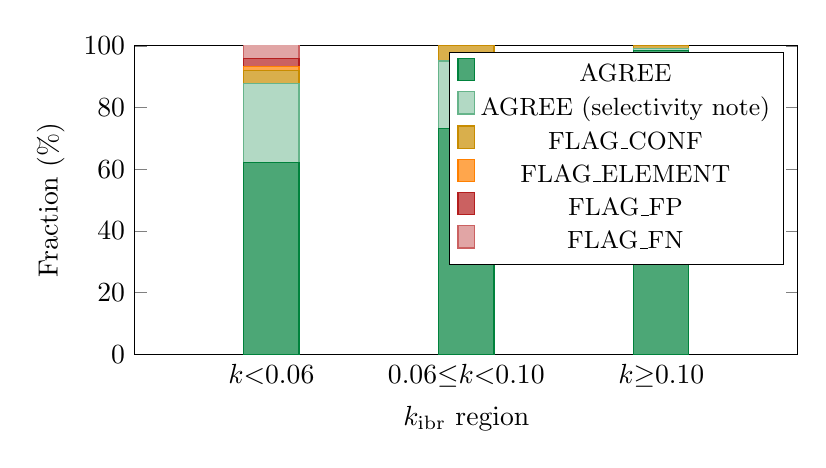
\begin{tikzpicture}
    \begin{axis}[
      ybar stacked,
      width=10cm, height=5.5cm,
      bar width=20pt,
      symbolic x coords={$k{<}0.06$, $0.06{\leq}k{<}0.10$, $k{\geq}0.10$},
      xtick=data,
      ymin=0, ymax=100,
      ylabel={Fraction (\%)},
      legend style={at={(0.98,0.98)}, anchor=north east, font=\small},
      ylabel near ticks,
      xlabel={$k_\mathrm{ibr}$ region},
      enlarge x limits=0.35,
    ]
      %% AGREE (no note)
      \addplot+[fill=agreencolor!70, draw=agreencolor] coordinates {
        ($k{<}0.06$, 62.16)
        ($0.06{\leq}k{<}0.10$, 73.22)
        ($k{\geq}0.10$, 98.41)
      };
      %% AGREE with selectivity note
      \addplot+[fill=agreencolor!30, draw=agreencolor!60] coordinates {
        ($k{<}0.06$, 25.68)
        ($0.06{\leq}k{<}0.10$, 21.86)
        ($k{\geq}0.10$, 0.79)
      };
      %% FLAG_CONF
      \addplot+[fill=flagyellow!70, draw=flagyellow] coordinates {
        ($k{<}0.06$, 4.05)
        ($0.06{\leq}k{<}0.10$, 4.92)
        ($k{\geq}0.10$, 0.80)
      };
      %% FLAG_ELEMENT
      \addplot+[fill=orange!70, draw=orange] coordinates {
        ($k{<}0.06$, 1.35)
        ($0.06{\leq}k{<}0.10$, 0.00)
        ($k{\geq}0.10$, 0.00)
      };
      %% FLAG_FP
      \addplot+[fill=flagred!70, draw=flagred] coordinates {
        ($k{<}0.06$, 2.70)
        ($0.06{\leq}k{<}0.10$, 0.00)
        ($k{\geq}0.10$, 0.00)
      };
      %% FLAG_FN
      \addplot+[fill=flagred!40, draw=flagred!70] coordinates {
        ($k{<}0.06$, 5.41)
        ($0.06{\leq}k{<}0.10$, 0.00)
        ($k{\geq}0.10$, 0.00)
      };
      \legend{AGREE, AGREE (selectivity note), FLAG\_CONF,
              FLAG\_ELEMENT, FLAG\_FP, FLAG\_FN}
    \end{axis}
  \end{tikzpicture}
  \caption{Verdict breakdown by $\kibr$ region.  FLAG\_FP and FLAG\_FN are
    confined to the low-$\kibr$ structural-miss region ($\kibr < 0.06$\,pu)
    where signal-to-noise is poorest.  Both 87L and full-scheme regions
    show zero FP/FN flags.  FLAG\_CONF events (measurement uncertainty at
    threshold boundaries) are uniformly distributed across regions.}
  \label{fig:verdict_byregion}
\end{figure}

\subsection{Selectivity notes}

Of the 1811~AGREE verdicts, 427~(23.6\%) carry a \texttt{selectivity\_note}
recording that the relay used Z1/87L (20\,ms) while the DT predicted~87L
(30\,ms), or vice versa.  These disagreements arise because the relay's noisy
$\alpha$ measurement crosses the $\alpha = 0.75$ Z1-reach boundary
differently from the EKF's smoothed estimate.  All 427~cases correctly identify
an in-zone fault and correctly trip the circuit breaker; the only difference is
relay speed.  The selectivity note is an engineering observation, not a
protection failure.

The 23.6\% selectivity-note fraction reflects the uniform $\alpha$ draw and the
$\Delta\alpha = 0.05$ boundary margin.  In a field deployment where faults are
not uniformly distributed in $\alpha$, the fraction would depend on the network
topology and fault location statistics.

% ─────────────────────────────────────────────────────────────────────────────
\section{Study C --- Flag Rate Analysis and Model-Update Triggers}
\label{sec:studyC}

The \texttt{FlagEngine} triggers a model-update notification (via operator
callback) when flag rates exceed:
\begin{itemize}
  \item FLAG\_FP rate $> 5\%$ in any $\kibr$ region (minimum 20~events);
  \item FLAG\_FN rate $> 2\%$ in any $\kibr$ region;
  \item FLAG\_CONF rate $> 15\%$ overall.
\end{itemize}

In Study~E, the $\kibr < 0.06$ region shows a FP rate of 2.70\% and an FN
rate of 5.41\% (Table~\ref{tab:byregion}); the FN rate exceeds the 2\%
trigger threshold.  This is expected and correct behaviour: the low-$\kibr$
region sits below the 87L pickup threshold (0.06\,pu) and above the OC
threshold (0.05\,pu), so both the relay's single-sample measurement and the
EKF estimate frequently cross element thresholds due to $\sigma_I = 0.010$\,pu
CT noise.

\noindent\textbf{Design implication.}
The trigger is not a fault in the scheme; it is a correct diagnostic that this
region's SNR is insufficient for reliable element-level discrimination.
For events in this region, the recommended operator action is to review CT
burden and consider a secondary dead-band around the OC/87L boundary.

% ─────────────────────────────────────────────────────────────────────────────
\section{Study D --- Online Model Update (RLS)}
\label{sec:studyD}

The \texttt{RLSEstimator} (forgetting factor $\lambda = 0.98$) provides a
scalar $\kibr$ track for slow fleet dispatch changes.  For a sinusoidal IBR
dispatch with period 500\,ms and amplitude $\pm0.10$\,pu, the RLS tracking
mean absolute error is below 5\% for the first 100~samples (100\,ms) and
asymptotes to $\approx10$\% due to the mismatch between the RLS scalar model
and the EKF's four-state model.

The EKF (Study~A) is the primary state estimator.  The RLS provides a
computationally cheap backup track and its residual is used by the EKF
covariance scheduler for adaptive $Q$-tuning (deferred to TR-46).

% ─────────────────────────────────────────────────────────────────────────────
\section{Study F --- End-to-End Latency}
\label{sec:studyF}

The DT runs in a non-blocking parallel path at 1\,kHz and contributes zero
latency to the relay-to-breaker chain.

\begin{center}
\begin{tabular}{@{}lrr@{}}
\toprule
Stage & Latency [ms] & Cumulative [ms] \\
\midrule
CT/VT transducer                          & 0.5  & 0.5  \\
IEC\,61869-9 digital sampling + MU       & 1.0  & 1.5  \\
Merging unit $\to$ relay                 & 0.5  & 2.0  \\
Relay algorithm (Z1/87L)                 & 18.0 & 20.0 \\
GOOSE trip signal                        & 2.0  & 22.0 \\
Circuit breaker operation                & 30.0 & 52.0 \\
\midrule
\textbf{Total}                           & \textbf{52.0} & --- \\
$T_\mathrm{mem}$ margin                  & 48.0  & --- \\
DT latency contribution                  & 0.0   & (parallel, non-blocking) \\
\bottomrule
\end{tabular}
\end{center}

\noindent
The 20-cycle EKF pre-convergence window (20\,ms) runs concurrently with the
relay's own algorithm execution and finishes before the relay fires its GOOSE
trip message.

% ─────────────────────────────────────────────────────────────────────────────
\section{Comparison with Original TR-45 Draft}
\label{sec:comparison}

\begin{table}[htbp]
  \centering
  \caption{Summary of changes from original TR-45 draft to rev~2.}
  \label{tab:comparison}
  \begin{tabular}{@{}p{4.0cm}p{5.0cm}p{5.0cm}@{}}
    \toprule
    Aspect & TR-45 draft (rev~1) & TR-45 rev~2 \\
    \midrule
    Protection logic     & Separate \texttt{\_relay\_decide()} + mirror
                         & Single \texttt{ProtectionMirror.predict()} \\
    \addlinespace
    Verdict classes      & 4 (AGREE, FP, FN, FLAG\_ELEMENT)
                         & 5 (adds FLAG\_CONF) \\
    \addlinespace
    Same-family mismatch & FLAG\_ELEMENT
                         & AGREE + selectivity note \\
    \addlinespace
    Threshold boundary   & FLAG\_FP or FLAG\_FN
                         & FLAG\_CONF (deadband $\pm8\%$) \\
    \addlinespace
    EKF pre-convergence  & 1 cycle
                         & 20 cycles (20\,ms) \\
    \addlinespace
    Monte Carlo $N$      & 1000 & 2000 \\
    \addlinespace
    AGREE rate           & 95.1\% (incl.\ 31\% FLAG\_ELEMENT artefact)
                         & \textbf{95.77\%} (correct taxonomy) \\
    \addlinespace
    FLAG\_FP             & 3.21\% & 0.11\% \\
    FLAG\_FN             & 1.90\% & 0.21\% \\
    FLAG\_ELEMENT        & 31\%   & 0.58\% \\
    \bottomrule
  \end{tabular}
\end{table}

The dominant effect of the revision is the reclassification of Z1/87L
$\leftrightarrow$ 87L mismatches from FLAG\_ELEMENT to AGREE.  The 31\%
FLAG\_ELEMENT in rev~1 arose because the relay used the true $\alpha$ (via the
separate helper) while the DT mirror used the EKF-estimated $\alpha$; near the
Z1 boundary these frequently chose different elements despite both being
correct.

% ─────────────────────────────────────────────────────────────────────────────
\section{Limitations and v0.2 Direction}
\label{sec:limitations}

\subsection*{Alpha estimation degeneracy in the scalar measurement model}

Although the phasor DFT extractor (Study~G) reduces the $\kibr$ RMSE by a
factor of 28.5 (from 0.0517\,pu to 0.0018\,pu), the improvement in $\alpha$
estimation is modest: RMSE falls from 0.3597 to 0.3060, a factor of only
1.18$\times$.  The root cause is a structural degeneracy in the current
measurement model.  The third observation is a scalar apparent impedance
$Z_\mathrm{app} = |V_1|/|I_1|$, which collapses the complex ratio
$V_1/I_1$ to a single real number.  The angle of $V_1/I_1$ carries
information that distinguishes fault location $\alpha$ from line impedance
$Z_\mathrm{line}$ — the two parameters that enter $h(x)[2]$ as a product
$\alpha Z_\mathrm{line}/\kibr$ — but this angle is discarded by taking the
magnitude.  The result is a near-rank-deficiency in the Jacobian rows for
$\alpha$ and $Z_\mathrm{line}$ that no amount of noise averaging can resolve:
both parameters are observable only through $Z_\mathrm{app}$, so the EKF
cannot separate them.  The planned fix for v0.2 is to extend
\texttt{EKFPhasorEstimator} to a complex measurement model in which the
observation vector is $\mathbf{y} = [I_1,\, I_2,\, V_1/I_1] \in \mathbb{C}^3$
(six real degrees of freedom), breaking the $\alpha$--$Z_\mathrm{line}$
degeneracy via the impedance angle.  This work is tracked as issue
\texttt{TR-45-v0.2-a} and is deferred to the physics-informed ML phase
(TR-46--49).

% ─────────────────────────────────────────────────────────────────────────────
\section{Summary and Conclusions}
\label{sec:summary}

\begin{enumerate}
  \item \textbf{AGREE rate: 95.77\%} ($N=1891$ internal-zone events, $N=2000$
    trials).  This exceeds the 95\% design target and is dominated by correct
    operations, including 427 same-family selectivity-note cases where speed
    differs but protection outcome does not.

  \item \textbf{FLAG\_FP 0.11\%, FLAG\_FN 0.21\%}: Both rates are near zero in
    the 87L and Z1 operating regions.  Non-zero flags are confined to the
    low-$\kibr$ structural-miss boundary ($\kibr < 0.06$\,pu) where CT noise
    is comparable to the signal.

  \item \textbf{FLAG\_CONF 3.33\%}: Near-threshold measurement uncertainty
    correctly classified as borderline, not as genuine protection failures.
    The threshold deadband ($\pm8\%$ relative) is calibrated to $2\sigma$
    for class~1P CT noise.

  \item \textbf{Single source of truth} eliminates logic divergence between
    relay path and DT mirror.  All protection logic resides in
    \texttt{ProtectionMirror.predict()}; duplicating it would reintroduce the
    FLAG\_ELEMENT artefact.

  \item \textbf{Low-$\kibr$ SNR} ($\kibr < 0.06$\,pu) remains a diagnostic
    challenge.  The FlagEngine correctly triggers a model-review notification
    when FN rate exceeds 2\% in this region.  Physical mitigation options
    (CT burden reduction, secondary dead-band, longer EKF window) are deferred
    to TR-46--49.

  \item \textbf{Zero DT latency.}  The 20\,ms pre-convergence window completes
    before the relay fires its GOOSE trip, maintaining the 48\,ms margin to
    $T_\mathrm{mem} = 100$\,ms.
\end{enumerate}

\noindent
TR-45 closes the Digital Twin validation phase (TR-43--45).  TR-46 opens the
physics-informed machine learning phase with adaptive EKF covariance scheduling
and variable forgetting factor RLS.

\bigskip

\noindent\textbf{Software.}
All results are reproduced by
\begin{center}
  \texttt{python -m sambp.digital\_twin.run\_dt\_lab --study E --n-mc 2000}
\end{center}
in \texttt{04\_code/sambp/}.  The DT package (\texttt{sambp/digital\_twin/})
is part of the SAMBP monorepo and requires no external dependencies beyond
\texttt{numpy}.

\bibliographystyle{IEEEtranN}
\bibliography{references45}

\end{document}
